\documentclass{article}


% if you need to pass options to natbib, use, e.g.:
%     \PassOptionsToPackage{numbers, compress}{natbib}
% before loading neurips_2023


% ready for submission
\usepackage[final, nonatbib]{neurips_2023}


% to compile a preprint version, e.g., for submission to arXiv, add add the
% [preprint] option:
%     \usepackage[preprint]{neurips_2023}


% to compile a camera-ready version, add the [final] option, e.g.:
%     \usepackage[final]{neurips_2023}


% to avoid loading the natbib package, add option nonatbib:
%    \usepackage[nonatbib]{neurips_2023}


\usepackage[utf8]{inputenc} % allow utf-8 input
\usepackage[T1]{fontenc}    % use 8-bit T1 fonts
\usepackage{hyperref}       % hyperlinks
\usepackage{url}            % simple URL typesetting
\usepackage{booktabs}       % professional-quality tables
\usepackage{amsfonts}       % blackboard math symbols
\usepackage{nicefrac}       % compact symbols for 1/2, etc.
\usepackage{microtype}      % microtypography
\usepackage{xcolor}         % colors

\usepackage[spanish, es-tabla]{babel}

\usepackage[pdftex]{graphicx}
\usepackage{subcaption}
\graphicspath{{./graphs/}}

%% biblatex
\usepackage[style = numeric, backend = biber, sorting = none, doi = false, isbn = false, url = true]{biblatex}
% \usepackage[defernumbers = true, style = numeric, backend = biber, sorting = none, doi = false, isbn = false, url = true]{biblatex}
% \usepackage[style = numeric, backend = biber, sorting = none]{biblatex}    % REFERENCIAS como section
\AtEveryBibitem{
    \clearfield{urlyear}
    \clearfield{urlmonth}
} % Do not show the "(visited on <date>)" on the references
\DefineBibliographyStrings{spanish}{}
\usepackage{csquotes}
\addbibresource{./dmcyt.bib}
\renewcommand*{\bibfont}{\fontsize{9}{12}\selectfont}



\title{Grafos en neurociencias (pre TP2)}

\author{
  Víctor A.~Bettachini\\ %\thanks{Use footnote for providing further information about author (webpage, alternative address)---\emph{not} for acknowledging funding agencies.} \\
  Datamining en ciencia y tecnología 2023\\
  Especialización en Explotación de Datos y Descubrimiento del Conocimiento\\
  \texttt{bettachini@gmail.com}
}


\begin{document}


\maketitle


\begin{abstract}
?
\end{abstract}


% Enunciado
% Se sugiere realizar la entrega en formato latex, pero en este caso va a ser optativo (en el TP ya es obligatorio, sugerimos que lo usen de práctica). Pueden acceder a formatos de distintas conferencias a través de Overleaf, en particular les sugerimos el formato de NeurIPS que es una de las conferencias más importantes en IA.
% Se sugiere un máx de 4 carillas (mín 2), no se debe incluir código a menos que sea algo esencial que hayan desarrollado ustedes (es preferible en este caso incluir el pseudo-código). Aclaración: No vamos a corregir código en la entrega.
% El pre TP es individual.


% \section{Introducción}

\section{Materiales y métodos}

\paragraph{Datos}
Se registró la señal de resonancia magnética funcional (fMRI) bajo distintos estadíos del sueño en distintas parcializaciones del cerebro. 
Para segmentos temporales se calculó el coeficiente de correlación lineal entre sus medias \cite{tagliazucchi_large-scale_2013}.
Estos son los datos de entrada con que se genera una matríz de correlación a partir de la cual se generan los grafos que se analizan en este trabajo.

\paragraph{Recurso informático} 
Un cuaderno (notebook) Jupyter provisto por los docentes en el sitio web denominado ``Campus'' \cite{kamienkowski_curso_2023} es la plantilla donde se escribió código en lenguaje Python.
Este explotó funciones de las biblioteca NetworkX \cite{hagberg_exploring_2008}.



\subsection{Preprocesamiento de los datos}
% Cada actividad realizada se describe bajo los titulos que figuran en el enunciado del trabajo práctico publicado en el

\paragraph{Carga del conjunto de datos} 
Los archivos provistos corresponden a los estadíos de sueño N1, N2, N3 y despierto (W) para 18 sujetos.
Estos estuvieron acompañados de una tabla que describe la denominacion y  ubicación espacial las regiones en que se parcializó el cerebro.



\section{Resultados}

\subsection{Manipulación de datos}

\paragraph{Matriz de correlación}
Para las regiones en que se parcializó el cerebro se obtuve la matriz de adyacencia pesada que muestra la figura \ref{fg:matriz_correlación_pesada}.
Para convertirle en una de adyacencia binaria con una densidad de enlaces \(\delta = 0.8\) se discriminaron sus pesos con un umbral \(0.77997\) obteníendose la matriz que muestra la figura \ref{fg:matriz_correlación_binaria}.

\begin{figure}[ht]
	\centering
	\begin{subfigure}[b]{0.4\textwidth}
		\includegraphics[width= \linewidth]{matriz_correlación}
		\caption{Pesada}
		\label{fg:matriz_correlación_pesada}
	\end{subfigure}
	\begin{subfigure}[b]{0.425\textwidth}
		\includegraphics[width= \linewidth]{matriz_correlación_binaria}
		\caption{Binaria}
		\label{fg:matriz_correlación_binaria}
	\end{subfigure}
	\caption{Matrices de correlación de las medias de las señales de las regiones parcializadas.
	}
	\label{fg:matriz_correlación}
\end{figure}


% \section{Discusión}

\begin{figure}[ht]
  \centering
  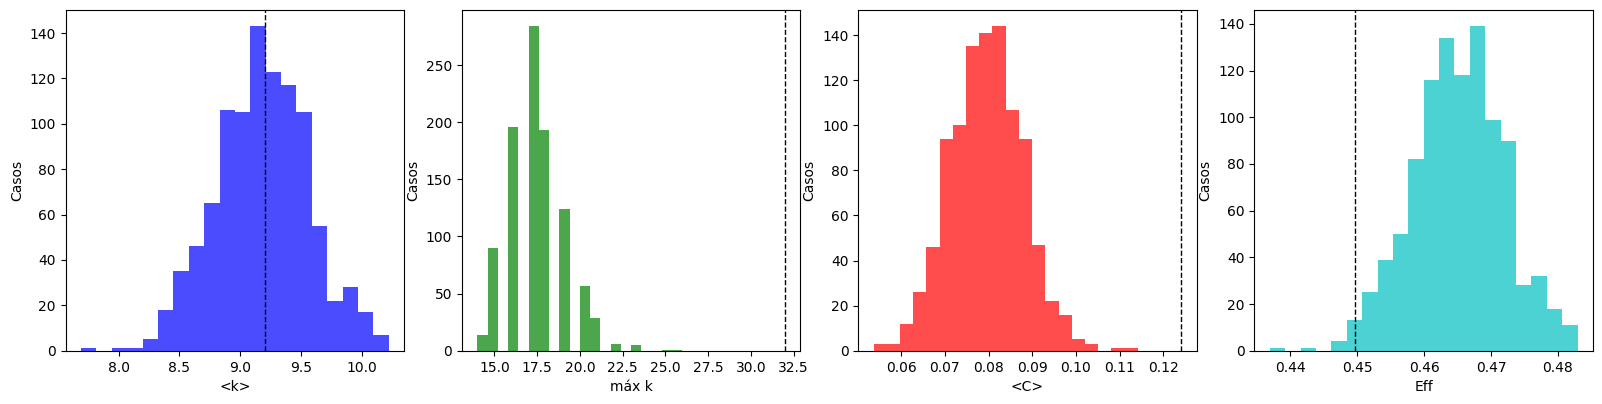
\includegraphics[width= \linewidth]{hist_poisson}
  \caption{Poisson
	}
	\label{fg:hist_poisson}
\end{figure}


\printbibliography[title= Referencias, heading=bibintoc]

\end{document}
